\documentclass[11pt,a4paper]{article}
\usepackage[margin=25mm]{geometry}
\usepackage{fontspec}
\setmainfont{TeX Gyre Pagella}
\usepackage{amsmath,amssymb,mathtools}
\usepackage{graphicx}
\usepackage{xcolor}
\usepackage[unicode,colorlinks=true,linkcolor=blue,urlcolor=blue]{hyperref}
\usepackage{bookmark}
\usepackage{enumitem}
\setlist{itemsep=3pt,topsep=5pt}
\setlength{\emergencystretch}{3em}
\newcommand{\tightlist}{\setlength{\itemsep}{0pt}\setlength{\parskip}{0pt}}
\newcommand{\passthrough}[1]{#1}
\newcommand{\pandocbounded}[1]{#1}
\makeatletter
\def\maxwidth{\ifdim\Gin@nat@width>\linewidth\linewidth\else\Gin@nat@width\fi}
\def\maxheight{\ifdim\Gin@nat@height>0.75\textheight0.75\textheight\else\Gin@nat@height\fi}
\makeatother
\setkeys{Gin}{width=\maxwidth,height=\maxheight,keepaspectratio}
\hypersetup{pdfauthor={OpenAI GPT-6.1 Sol, Codex, Ultra effort}}
\begin{document}
\section{Profinite groups and infinite Galois
theory}\label{profinite-groups-and-infinite-galois-theory}

\emph{Written by OpenAI GPT-6.1 Sol in Codex, Ultra effort, October
2026. Self-checked by the writing AI; no independent review is claimed.
Public domain (CC0).}

An automorphism of an infinite algebraic extension is determined by its
actions on finite subextensions. These actions cannot be chosen
independently: restricting an action from a larger field must recover
the action already chosen on a smaller one. This compatibility turns an
infinite Galois group into a compact topological group. Class field
theory will describe its abelian quotients by arithmetic data.

We use field operations, polynomial division, finite-dimensional linear
algebra and the basic definitions of compact Hausdorff spaces and
product topology. Section 0 proves the finite Galois correspondence and
the Chinese remainder theorem used below. We also prove the required
compactness and multiquadratic facts. The irreducibility and finite
Galois groups of cyclotomic polynomials are proved in
\href{https://kokunoyumeto.github.io/open-math-courses/courses/NT-CFT/cyclotomic-polynomials-and-their-automorphisms.html}{Cyclotomic
fields}, Theorem 12.1. Here we use that theorem to pass to infinite
extensions. Freely accessible comparisons are Milne's \emph{Fields and
Galois Theory} and Kedlaya's \emph{Notes on class field theory}.

\textbf{Prerequisite proof availability.} The named results below
identify specific programme lessons. The
\href{https://kokunoyumeto.github.io/open-math-courses/courses/NT-CFT/proof-dependencies.html\#lesson-1}{prerequisite
record} distinguishes published proofs, supplied owner texts awaiting
publication, and missing full proofs. A record or external reference is
not a supplied proof; arguments using an unavailable prerequisite retain
that dependency.

\subsection{0. The finite algebra behind the
limits}\label{the-finite-algebra-behind-the-limits}

We first establish the algebraic results needed to recover an infinite
field from its finite pieces.

\textbf{Finite automorphism lemma.} If a finite group \(H\) of distinct
automorphisms acts on a field \(E\), and \(F=E^H\), then \([E:F]=|H|\).
Moreover \(E/F\) is separable and normal, and \(H\) is its full
automorphism group.

\textbf{Proof.} Put \(n=|H|\). Given \(n+1\) elements
\(x_1,\ldots,x_{n+1}\) of \(E\), form the matrix with entries
\(h(x_j)\), indexed by \(h\in H\). Its homogeneous system has a nonzero
solution over \(E\). Choose a solution \(c=(c_j)\) with least possible
nonzero support and scale one nonzero coordinate to 1. Applying any
\(h_0\in H\) to every equation permutes the rows, so \(h_0(c)\) is
another solution. The difference \(h_0(c)-c\) has smaller support,
because the normalized coordinate vanishes. Minimality forces this
difference to be zero. Thus every \(c_j\) belongs to \(F\), and the
identity row gives a nontrivial \(F\)-linear dependence among the
\(x_j\). Consequently \(d=[E:F]\leq n\).

Distinct field homomorphisms are linearly independent over the target
field. Indeed, a nontrivial relation with least number of terms cannot
have one term. If \(h_1\) and \(h_r\) occur, select \(y\) with
\(h_1(y)\ne h_r(y)\). Subtract \(h_r(y)\) times the relation evaluated
at \(x\) from the relation evaluated at \(yx\). This removes the last
term and leaves the first nonzero, contradicting minimality. Each member
of \(H\) is \(F\)-linear, while \(\operatorname{Hom}_F(E,E)\) has
dimension \(d\) over \(E\): evaluation on an \(F\)-basis identifies it
with \(E^d\). Hence \(n\leq d\), proving equality.

For \(x\in E\), multiply \(X-z\) over the distinct members \(z\) of its
\(H\)-orbit. The resulting polynomial is fixed coefficientwise by \(H\),
hence belongs to \(F[X]\), and has distinct roots in \(E\). The minimal
polynomial of \(x\) over \(F\) divides it. Thus that minimal polynomial
is separable and splits in \(E\). This proves both separability and
normality.

Finally a finite extension of degree \(d\) has at most \(d\) embeddings
into an algebraic closure. To prove the bound, choose finitely many
generators and adjoin them successively; at each step an embedding has
at most the minimal-polynomial degree many extensions, since the new
generator must go to one of its roots. Multiplying these bounds gives
the extension degree by the tower law. Since the \(n=d\) members of
\(H\) already attain the bound, there are no other automorphisms.
\(\square\)

For a finite separable extension the same generator argument gives
exactly the degree many embeddings: at each stage the transformed
minimal polynomial has its full number of distinct roots in an algebraic
closure, and sending the generator to any of them defines an extension
of the embedding. If the extension is normal, all these embeddings
preserve the field and are automorphisms. Preservation implies
surjectivity because the image has the same finite dimension over the
ground field.

\textbf{Finite Galois correspondence.} Let \(E/K\) be finite, separable
and normal, with group \(G\). Subgroups \(H\subset G\) correspond
bijectively and in reverse inclusion order to intermediate fields, by \[
H\longmapsto E^H,\qquad M\longmapsto\operatorname{Gal}(E/M).
\] The degree is \([E^H:K]=[G:H]\). Normal subgroups correspond to
normal extensions of \(K\), with quotient group \(G/H\).

\textbf{Proof.} The automorphism lemma gives
\(\operatorname{Gal}(E/E^H)=H\) and \([E:E^H]=|H|\). For an intermediate
field \(M\), the extension \(E/M\) is still separable and normal: the
minimal polynomial over \(M\) of any element of \(E\) divides its split
separable polynomial over \(K\). The embedding count gives
\(|\operatorname{Gal}(E/M)|=[E:M]\). Its fixed field contains \(M\), and
the automorphism lemma gives it the same relative degree as \(M\), so
the fields are equal. The tower law proves the displayed degree formula.

A \(K\)-embedding of \(M\) into an algebraic closure extends to an
embedding of \(E\) by the successive root construction. Normality of
\(E/K\) makes the extension an element of \(G\). It follows that \(M/K\)
is normal exactly when \(M\) is preserved by every element of \(G\). The
equality \(g(E^H)=E^{gHg^{-1}}\), and the bijection just proved, make
this equivalent to normality of \(H\). In that case restriction maps
\(G\) onto \(\operatorname{Gal}(M/K)\), with kernel \(H\), proving the
quotient assertion. \(\square\)

\textbf{Primitive element lemma.} A finite separable extension \(E/K\)
is generated by one element. For infinite \(K\), write
\(E=K(a_1,\ldots,a_r)\), and list its \(d=[E:K]\) embeddings into an
algebraic closure, as counted above. For each pair of different
embeddings, the linear polynomial \(\sum_j c_j(\sigma(a_j)-\tau(a_j))\)
is nonzero. Their product is a nonzero polynomial in the \(c_j\). A
nonzero polynomial over an extension of an infinite field cannot vanish
on every tuple from that field: induction on the number of variables
chooses values at which a nonzero coefficient stays nonzero, and then
avoids finitely many roots in the last variable. Choose \(c_j\in K\)
making this product nonzero. The element \(a=\sum_j c_ja_j\) then has
\(d\) distinct images. Its minimal polynomial has degree at least \(d\),
and at most \([E:K]=d\); thus \(K(a)=E\).

For finite \(K\), the field \(E\) is finite. Its multiplicative group is
cyclic. To prove this, let \(m\) be its exponent. For each prime power
dividing \(m\), choose an element attaining that prime-power order by
taking a suitable power of an element whose order contains it. The
product of these elements has order \(m\), because they commute and
their orders are pairwise coprime. Every nonzero element is a root of
\(X^m-1\), so the polynomial root bound gives \(|E^\times|\leq m\).
Since \(m\) divides the group order, equality follows. A generator of
\(E^\times\) consequently generates \(E\) as a field. This proves the
lemma in both cases.

\textbf{Chinese remainder lemma.} For pairwise coprime positive integers
\(n_1,\ldots,n_r\), reduction gives \[
\mathbf Z/(n_1\cdots n_r)\mathbf Z
\simeq\prod_{j=1}^r\mathbf Z/n_j\mathbf Z.
\] Put \(N=n_1\cdots n_r\). For each \(j\), Bezout's identity supplies
integers \(b_j,c_j\) with \(b_j(N/n_j)+c_jn_j=1\). Then \(e_j=b_jN/n_j\)
has residue 1 at \(n_j\) and 0 at the other moduli. Thus
\(\sum_j a_je_j\) lifts any desired tuple of residues. An integer in the
kernel is divisible by every \(n_j\), hence by their product, proving
injectivity. The divisibility assertion follows successively from
Bezout: if \(a,b\) are coprime and both divide \(x\), then \(b\) divides
\(x/a\). Bezout itself follows by choosing the least positive integer in
the ideal \((a,b)\) and applying integer division to show that it
divides both generators. This also proves the construction without
assuming the remainder lemma in advance.

The same construction proves the \textbf{polynomial remainder lemma}
used later for completions: if \(f_1,\ldots,f_r\in k[X]\) are pairwise
coprime, then \[
k[X]/(f_1\cdots f_r)\simeq\prod_j k[X]/(f_j).
\] Polynomial division shows that an ideal generated by two polynomials
is generated by a polynomial of least nonzero degree: division by that
polynomial leaves a smaller-degree member of the ideal, hence zero.
Coprimality therefore gives a polynomial Bezout identity. Apply it to
\(f_j\) and the product of the other factors to construct the same
idempotent lifts as above. An element in the kernel is divisible by each
factor, and successive Bezout identities make it divisible by the
product. This proves surjectivity and injectivity over every field
\(k\).

\subsection{1. What compatibility means}\label{what-compatibility-means}

For every positive integer \(n\), put

\[
\widehat{\mathbf Z}=\varprojlim_n\mathbf Z/n\mathbf Z.
\]

The indexing order is divisibility. An element is a family \((a_n)_n\),
with \(a_n\in\mathbf Z/n\mathbf Z\), satisfying \(a_m\bmod n=a_n\)
whenever \(n\mid m\). Addition and multiplication are coordinatewise.
Give each finite ring its discrete topology and the limit the subspace
topology of their product.

The map \(\mathbf Z\to\widehat{\mathbf Z}\) is injective: an integer
divisible by every positive integer is zero. Its image is dense. Indeed,
finitely many compatible congruence conditions are all satisfied by an
integer representing the coordinate at the least common multiple of
their moduli.

Over \(\mathbf F_q\), restriction from \(\mathbf F_{q^m}\) to
\(\mathbf F_{q^n}\), for \(n\mid m\), takes the exponent of the
Frobenius automorphism modulo \(m\) to that exponent modulo \(n\). Thus
compatible Frobenius exponents give exactly this inverse limit. Notice
that the algebraic cyclic subgroup generated by Frobenius contains only
integral exponents. Taking its closure adds all compatible profinite
exponents.

The same construction works for an inverse system of finite groups
\(G_i\) with homomorphisms \(G_j\to G_i\). Its inverse limit consists of
the compatible tuples in \(\prod_iG_i\). A \textbf{profinite group} is a
topological group isomorphic to such an inverse limit.

\begin{figure}
\centering
\pandocbounded{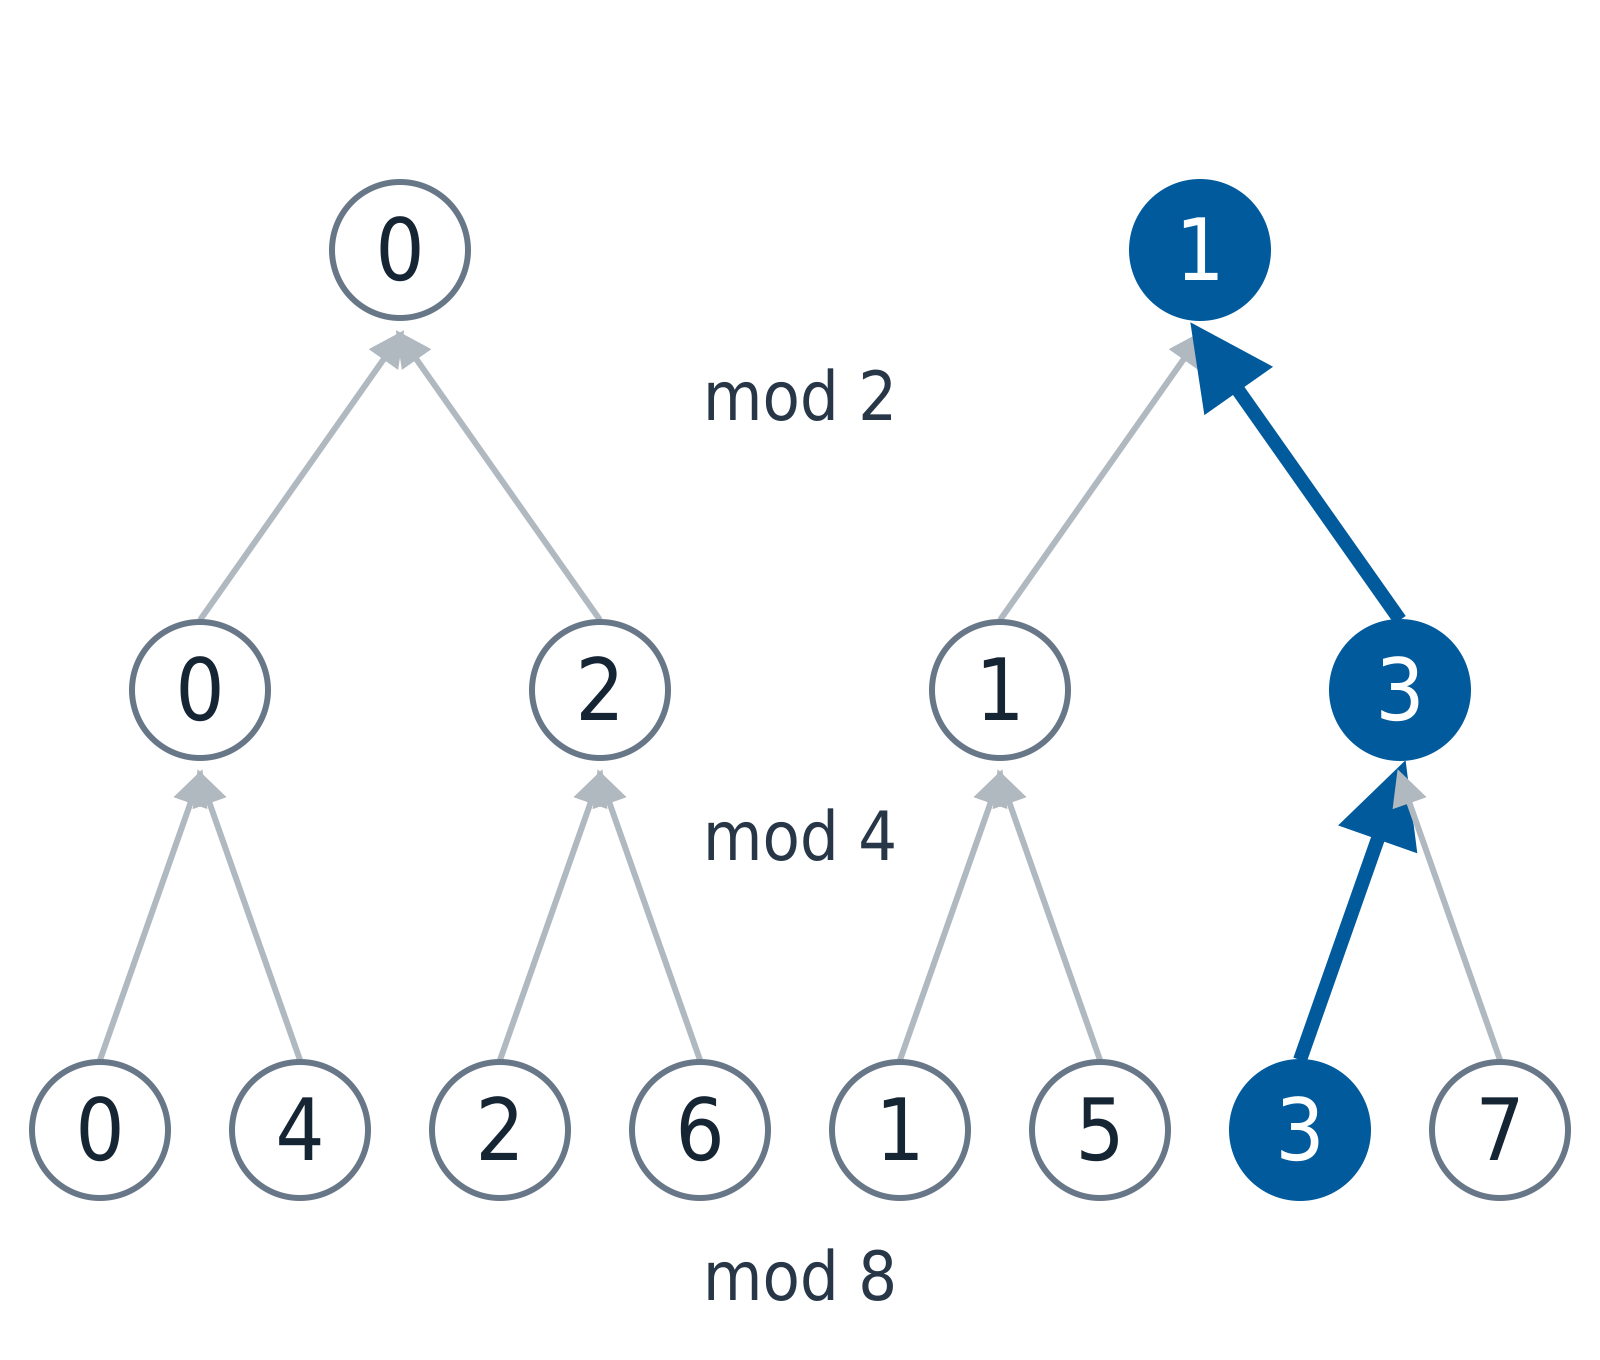
\includegraphics[keepaspectratio,alt={Three finite stages of the 2-adic inverse limit. Each residue modulo 8 maps to its residue modulo 4, then modulo 2. The highlighted compatible residues are 3, 3 and 1.}]{assets/compatible-residues.png}}
\caption{Three finite stages of the 2-adic inverse limit. Each residue
modulo 8 maps to its residue modulo 4, then modulo 2. The highlighted
compatible residues are 3, 3 and 1.}
\end{figure}

\emph{Figure 1. Finite approximations to \(\mathbf Z_2\). Each edge is
reduction of a residue. The highlighted branch is the image of the
integer 3. Continuing the tree indefinitely gives \(\mathbf Z_2\); this
finite drawing is a schematic of the compatibility condition.}

\subsection{2. Finite quotients recognize compact
groups}\label{finite-quotients-recognize-compact-groups}

\subsubsection{Proposition 1.1. Characterization of profinite
groups}\label{proposition-1.1.-characterization-of-profinite-groups}

A topological group is profinite if and only if it is compact, Hausdorff
and totally disconnected. In a profinite group, open normal subgroups
form a neighborhood basis at the identity. Every open subgroup is closed
and has finite index. Conversely, every closed subgroup of finite index
is open.

\textbf{Proof.} First, a product of finite discrete nonempty spaces is
compact. To see this directly, take a family of closed subsets with the
finite intersection property. The filter it generates extends to a
maximal proper filter, or ultrafilter, by Zorn's lemma. In a finite
partition, exactly one part belongs to an ultrafilter: two disjoint
parts cannot both belong, and if no part belonged then all their
complements would belong, giving an empty intersection. Apply this to
each coordinate partition and choose its selected coordinate value. The
tuple so obtained has every basic neighborhood in the ultrafilter. It
belongs to each original closed set, because otherwise its open
complement would contain such a neighborhood and contradict membership
of that closed set in the filter. Thus every closed family with the
finite intersection property has nonempty intersection, the equivalent
closed-set formulation of compactness. A product containing an empty
factor is empty and compact as well. Products of Hausdorff spaces are
Hausdorff, since a differing coordinate separates two points.

An inverse limit of finite discrete groups is a closed subset of their
product: each compatibility condition is an equality of two continuous
maps to a finite Hausdorff space. It is consequently compact and
Hausdorff. Any two distinct tuples differ at a coordinate, and that
coordinate separates them by a clopen set. A connected subset can
therefore have only one point. Finite intersections of coordinate
kernels form a basis of open normal subgroups.

For the converse, we first justify the clopen neighborhoods that total
disconnectedness supplies. In a compact Hausdorff space \(X\), let
\(Q_x\) be the intersection of all clopen sets containing \(x\). This
intersection is connected. Otherwise write it as two disjoint nonempty
compact sets, with \(x\) in the first, and choose disjoint open
neighborhoods \(U,V\) of those sets. Each point outside \(U\cup V\) is
excluded by a clopen neighborhood of \(x\). Compactness gives finitely
many such neighborhoods whose intersection \(C\) lies in \(U\cup V\).
Both \(C\cap U\) and \(C\cap V\) are clopen in \(X\). The first contains
\(x\) and excludes the second part of \(Q_x\), contradicting the
definition of \(Q_x\). In a totally disconnected space it follows that
\(Q_x=\{x\}\). Applying compactness once more to the complement of any
neighborhood of \(x\) produces a clopen neighborhood inside it.

Now let \(G\) be compact, Hausdorff and totally disconnected, and choose
a clopen neighborhood \(C\) of 1 inside a prescribed neighborhood.
Compactness of \(C\) and continuity of multiplication give an identity
neighborhood \(V\) such that \(VC\subset C\). Replace \(V\) by a
symmetric smaller neighborhood. For \(g\in V\), both \(gC\subset C\) and
\(g^{-1}C\subset C\), so \(gC=C\). The stabilizer

\[
H=\{g\in G:gC=C\}
\]

is a subgroup containing \(V\), hence open; also \(H\subset C\), since
\(1\in C\). Its cosets form an open cover of the compact space \(G\), so
there are finitely many. The core \(N=\bigcap_{g\in G}gHg^{-1}\) is an
intersection of finitely many conjugates, and is an open normal subgroup
inside \(C\).

The natural map

\[
G\longrightarrow\varprojlim_{N\text{ open normal}}G/N
\]

is injective because these \(N\) form a basis and \(G\) is Hausdorff. It
is surjective: the cosets prescribed by a compatible tuple have the
finite intersection property, and compactness supplies a point in their
intersection. A continuous bijection from a compact space to a Hausdorff
space is a homeomorphism.

Finally, an open subgroup has open cosets; its complement is a union of
them, so it is closed. Compactness makes its index finite. If a subgroup
is closed and has finite index, its complement is a finite union of
closed cosets, so it is open. \(\square\)

The word \emph{closed} in the last assertion matters. We will construct
a subgroup of index 2 which is dense and proper.

\subsection{3. The correspondence for an infinite
extension}\label{the-correspondence-for-an-infinite-extension}

Let \(L/K\) be algebraic, normal and separable. Every finite collection
of elements of \(L\) lies in a finite Galois extension \(E/K\) contained
in \(L\): take the splitting fields of their minimal polynomials and
their compositum. Give \(G=\operatorname{Gal}(L/K)\) the \textbf{Krull
topology}, with the groups \(\operatorname{Gal}(L/E)\), for such \(E\),
as an identity neighborhood basis.

Restriction induces a topological isomorphism

\[
G\simeq\varprojlim_{E/K\text{ finite Galois in }L}\operatorname{Gal}(E/K).
\]

It is injective because the fields \(E\) exhaust \(L\). Conversely, a
compatible family defines an automorphism on their union; its inverse is
the family of inverse automorphisms. This also proves that the topology
just defined is the inverse-limit topology. In particular, \(G\) is
profinite.

Here is the embedding extension argument in the infinite case. In an
algebraic closure \(\Omega\) of \(K\), partially order embeddings of
subfields containing an intermediate field \(M\), extending a specified
\(K\)-embedding of \(M\), by extension of both domain and map. The union
along a chain is an embedding of its union field. Zorn's lemma supplies
a maximal embedding. If its domain omits \(x\in\Omega\), transform the
minimal polynomial of \(x\) by that embedding and choose a root in
\(\Omega\). Polynomial division identifies the adjoining field with the
quotient by the minimal polynomial, so this choice extends the embedding
to include \(x\), a contradiction. Its domain is therefore all of
\(\Omega\).

The image is algebraically closed: pull a polynomial's coefficients back
to \(\Omega\), split it there, and apply the embedding to its roots. It
contains \(K\), and every element of \(\Omega\) is algebraic over \(K\).
Its polynomial over \(K\) already splits in this image, so that element
belongs to the image. Hence the extended embedding is an automorphism of
\(\Omega\). Normality makes it and its inverse preserve \(L\), so
restriction gives an automorphism of \(L\). In particular,
\(G\to\operatorname{Gal}(E/K)\) is surjective for every finite Galois
\(E/K\) inside \(L\).

\subsubsection{Theorem 1.2. Infinite Galois
correspondence}\label{theorem-1.2.-infinite-galois-correspondence}

The assignments

\[
H\longmapsto L^H,
\qquad M\longmapsto\operatorname{Gal}(L/M)
\]

are inverse, inclusion-reversing bijections between closed subgroups of
\(G\) and fields \(K\subset M\subset L\). An open subgroup corresponds
to a finite extension of \(K\), with \([M:K]=[G:H]\). A closed normal
subgroup corresponds to a Galois extension of \(K\), and

\[
\operatorname{Gal}(M/K)\simeq G/H
\]

as topological groups. For any subgroup \(H\), closed or otherwise,

\[
\operatorname{Gal}(L/L^H)=\overline H.
\]

\textbf{Proof.} The group fixing \(M\) is closed: it is the intersection
of the stabilizers of its elements, and each stabilizer is open and
closed. If \(x\in L\setminus M\), the separable minimal polynomial of
\(x\) over \(M\) has another root in \(L\), since \(L/M\) is normal. The
embedding sending \(x\) to that root extends to an automorphism of
\(L/M\). Thus the fixed field of \(\operatorname{Gal}(L/M)\) is exactly
\(M\).

The action on each element of \(L\) is locally constant, so \(H\) and
\(\overline H\) have the same fixed field. If
\(\sigma\notin\overline H\), choose finite Galois \(E/K\) such that the
coset \(\sigma\operatorname{Gal}(L/E)\) misses \(H\). The restriction
\(\sigma|_E\) is outside the image \(H_E\) of \(H\) in
\(\operatorname{Gal}(E/K)\). Finite Galois theory supplies an element of
\(E^{H_E}\) moved by \(\sigma\). That element lies in \(L^H\). This
proves the last displayed equality and the bijection for closed
subgroups.

If \(H\) is open, it contains \(\operatorname{Gal}(L/E)\) for some
finite Galois \(E/K\). Hence \(L^H\subset E\), and finite Galois theory
computes its degree as \([G:H]\). Conversely, if \(M/K\) is finite,
finitely many generators have an open common stabilizer, namely
\(\operatorname{Gal}(L/M)\).

Conjugation gives \(L^{\sigma H\sigma^{-1}}=\sigma(L^H)\). Thus \(H\) is
normal exactly when \(M=L^H\) is stable under all \(K\)-automorphisms of
\(L\). By the extension fact, stability is equivalent to normality of
\(M/K\); separability is inherited. Restriction to \(M\) is then a
continuous surjection with kernel \(H\). Its quotient isomorphism is a
homeomorphism by compactness. \(\square\)

For two intermediate fields, taking their compositum corresponds to
intersecting their closed subgroups. Taking their intersection
corresponds to the closure of the subgroup generated by the two
subgroups. These follow directly from the inclusion-reversing bijection.

\subsection{4. Frobenius and cyclotomic
characters}\label{frobenius-and-cyclotomic-characters}

Inside an algebraic closure of \(\mathbf F_q\), the roots of
\(X^{q^n}-X\) form a field: raising to \(q^n\) preserves sums and
products in characteristic \(p\), and also preserves inverses of nonzero
roots. The derivative is \(-1\), so there are exactly \(q^n\) roots.
This gives a field of degree \(n\) over \(\mathbf F_q\). Conversely, a
degree-\(n\) extension has \(q^n\) elements and every nonzero element
satisfies \(x^{q^n-1}=1\) by the finite-group order theorem. It is
therefore exactly this root field. Its Frobenius has order \(n\): its
\(n\)-th power is the identity, while a smaller positive power \(d<n\)
cannot fix all \(q^n\) elements, since \(X^{q^d}-X\) has at most \(q^d\)
roots. The splitting-field extension is separable and Galois of degree
\(n\), so these \(n\) powers account for its entire Galois group. This
also shows that \(\mathbf F_{q^n}\subset\mathbf F_{q^m}\) exactly when
\(n\mid m\), using the tower law for necessity and iterated Frobenius
for sufficiency.

\subsubsection{Proposition 1.3. Two explicit infinite Galois
groups}\label{proposition-1.3.-two-explicit-infinite-galois-groups}

Arithmetic Frobenius \(x\mapsto x^q\) corresponds to 1 under

\[
\operatorname{Gal}(\overline{\mathbf F}_q/\mathbf F_q)\simeq\widehat{\mathbf Z}.
\]

The cyclotomic character gives topological isomorphisms

\[
\begin{aligned}
\operatorname{Gal}(\mathbf Q(\mu_\infty)/\mathbf Q)&\simeq\widehat{\mathbf Z}^{\times},\\
\operatorname{Gal}(\mathbf Q(\mu_{p^\infty})/\mathbf Q)&\simeq\mathbf Z_p^{\times}.
\end{aligned}
\]

The first character is characterized by
\(\sigma(\zeta)=\zeta^{\chi(\sigma)}\) for every root of unity
\(\zeta\).

\textbf{Proof.} Every finite extension of \(\mathbf F_q\) is
\(\mathbf F_{q^n}\), with cyclic Galois group of order \(n\) generated
by arithmetic Frobenius. Restriction reduces the exponent, giving the
first assertion and the density of the integral powers of Frobenius.

For each \(n\), cyclotomic irreducibility identifies
\(\operatorname{Gal}(\mathbf Q(\mu_n)/\mathbf Q)\) with
\((\mathbf Z/n\mathbf Z)^\times\). Restrictions are reductions of the
exponent. An element of \(\widehat{\mathbf Z}\) is a unit exactly when
every coordinate is a unit: the coordinatewise inverses are then
compatible. Infinite Galois theory therefore gives the second assertion.
Restricting to \(n=p^r\) gives the third. \(\square\)

The Chinese remainder theorem also gives

\[
\widehat{\mathbf Z}\simeq\prod_p\mathbf Z_p,
\qquad
\widehat{\mathbf Z}^{\times}\simeq\prod_p\mathbf Z_p^{\times}.
\]

The cyclotomic character is an action on roots of unity. It is not a
reciprocity map. Later, with arithmetic Frobenius as our reciprocity
convention, a finite unit idèle \(u\) over \(\mathbf Q\) will act on
roots of unity by the exponent \(u^{-1}\). Keeping this distinction
avoids a sign error in explicit reciprocity.

\subsection{5. A procyclic tower inside the cyclotomic
field}\label{a-procyclic-tower-inside-the-cyclotomic-field}

We need some elementary structure of local units. For odd \(p\),
simple-root lifting of \(X^{p-1}-1\) gives a subgroup
\(\mu_{p-1}\subset\mathbf Z_p^\times\) mapping isomorphically onto
\(\mathbf F_p^\times\). At each lifting step, the derivative is a unit,
so a unique correction modulo the next power of \(p\) exists.
Consequently

\[
\mathbf Z_p^\times=\mu_{p-1}\times(1+p\mathbf Z_p).
\]

The second factor is topologically isomorphic to the additive group
\(\mathbf Z_p\). Indeed, the binomial theorem gives

\[
v_p((1+p)^{p^r}-1)=r+1.
\]

For the inductive step, if \(v_p(t)\geq1\), then \(pt\) is the unique
lowest-valuation term of \((1+t)^p-1\). Hence the powers of \(1+p\)
generate every quotient \((1+p\mathbf Z_p)/(1+p^{r+1}\mathbf Z_p)\), of
order \(p^r\). The compatible exponent maps yield the desired
isomorphism.

For \(p=2\), reduction modulo 4 gives

\[
\mathbf Z_2^\times=\{\pm1\}\times(1+4\mathbf Z_2).
\]

Here \(v_2(5^{2^r}-1)=r+2\): squaring \(1+t\), with \(v_2(t)\geq2\),
increases \(v_2(t)\) by one. Thus 5 generates the finite quotients of
\(1+4\mathbf Z_2\), and this factor is again isomorphic to
\(\mathbf Z_2\).

\subsubsection{Proposition 1.4. The cyclotomic procyclic
extension}\label{proposition-1.4.-the-cyclotomic-procyclic-extension}

Let \(T\) be the closure of the finite-order elements of
\(\widehat{\mathbf Z}^\times\), and let \(\widetilde{\mathbf Q}\) be its
fixed field in \(\mathbf Q(\mu_\infty)\). Then

\[
\operatorname{Gal}(\widetilde{\mathbf Q}/\mathbf Q)\simeq\widehat{\mathbf Z}.
\]

For every number field \(K\), the compositum \(K\widetilde{\mathbf Q}\)
is Galois over \(K\) with Galois group topologically isomorphic to
\(\widehat{\mathbf Z}\).

\textbf{Proof.} The unit decompositions above give

\[
\widehat{\mathbf Z}^\times\simeq
\left(\{\pm1\}\times\prod_{p\text{ odd}}\mu_{p-1}\right)
\times\prod_p\mathbf Z_p.
\]

Write the first parenthesis as \(T_0\). The additive factors
\(\mathbf Z_p\) have no nonzero torsion, so every finite-order element
lies in \(T_0\). The finite-support elements of \(T_0\) all have finite
order and are dense in \(T_0\). Hence \(T=T_0\). The quotient is
\(\prod_p\mathbf Z_p\simeq\widehat{\mathbf Z}\), and Theorem 1.2 proves
the first assertion. Elements of \(T_0\) with infinitely many nontrivial
coordinates can have infinite order; this is why the closure is
essential.

Set \(E=K\cap\widetilde{\mathbf Q}\). This is finite over \(\mathbf Q\).
Restriction identifies \(\operatorname{Gal}(K\widetilde{\mathbf Q}/K)\)
with \(\operatorname{Gal}(\widetilde{\mathbf Q}/E)\). To justify
surjectivity even when \(K/\mathbf Q\) is not Galois, the image is
compact and hence closed, and its fixed field in
\(\widetilde{\mathbf Q}\) is \(E\); Theorem 1.2 therefore identifies the
image with that whole group.

A subgroup of index \(f\) in \(\widehat{\mathbf Z}\) which is open is
\(f\widehat{\mathbf Z}\). In fact it contains some
\(m\widehat{\mathbf Z}\), and its image in the cyclic group
\(\mathbf Z/m\mathbf Z\) is the unique subgroup of the indicated index.
Multiplication by \(f\) is an injective continuous map from
\(\widehat{\mathbf Z}\) onto \(f\widehat{\mathbf Z}\), and is a
homeomorphism by compactness. Apply this with \(f=[E:\mathbf Q]\).
\(\square\)

The extension \(\widetilde{\mathbf Q}\) is specified canonically as a
fixed field. An isomorphism of its Galois group with
\(\widehat{\mathbf Z}\) requires choices of generators of the local
principal-unit factors. In particular, there is no distinguished global
Frobenius generator here.

\subsection{6. Abelianization and a warning about finite
index}\label{abelianization-and-a-warning-about-finite-index}

For a profinite group \(G\), define

\[
G^{\mathrm{ab}}=G/\overline{[G,G]}.
\]

The closure is a closed normal subgroup, and the quotient is profinite
and abelian. Every continuous homomorphism from \(G\) to a Hausdorff
abelian group annihilates the commutators and their closure, so it
factors through this quotient.

For the absolute Galois group \(G_K\), its fixed field is
\(K^{\mathrm{ab}}\), the compositum of the finite abelian extensions in
a chosen separable closure. Indeed, each such extension corresponds to
an open normal subgroup containing the commutators. Conversely, the
profinite abelian quotient is the inverse limit of its finite abelian
quotients, whose fixed fields exhaust this compositum. A finite
compositum of abelian extensions is abelian because its Galois group
injects into the product of their abelian Galois groups.

We first justify the finite multiquadratic calculation needed for a
counterexample. For distinct primes \(p_1,\ldots,p_m\), put
\(E_m=\mathbf Q(\sqrt{p_1},\ldots,\sqrt{p_m})\). We claim that
\([E_m:\mathbf Q]=2^m\), with a basis consisting of the products
\(\prod_{i\in I}\sqrt{p_i}\), and that every choice of signs is a Galois
automorphism. Induct on \(m\), starting with \(E_0=\mathbf Q\). By the
induction hypothesis, the basis products in \(E_m\) have distinct
characters under its sign-change group. If \(x\in E_m\) has
\(x^2\in\mathbf Q^\times\), then every automorphism sends \(x\) to \(x\)
or \(-x\). Expanding in that basis shows that \(x\) lies in one
character space, hence is a rational multiple of one basis product. In
particular, \(\sqrt{p_{m+1}}\) cannot belong to \(E_m\): squaring such
an expression would contradict its odd valuation at the new prime.
Adjoining it therefore doubles the degree and gives the asserted basis.
The new extension is a splitting field of the polynomials \(X^2-p_i\),
so is Galois. Its group injects into the sign choices, and both sets
have \(2^{m+1}\) elements, so all sign choices occur. This completes the
induction.

Now consider

\[
L=\mathbf Q(\sqrt p:p\text{ prime}),
\qquad \operatorname{Gal}(L/\mathbf Q)\simeq\prod_p\mathbf F_2.
\]

The calculation just proved permits independent sign changes at each
finite stage; its restriction maps simply forget signs. Passage to the
inverse limit gives the displayed group.

Let \(V=\prod_p\mathbf F_2\), and let \(D=\bigoplus_p\mathbf F_2\) be
the finite-support subgroup. It is dense and proper. The quotient
\(V/D\) is a nonzero vector space. Choose a basis containing the class
of the all-ones vector, and define a linear functional to
\(\mathbf F_2\) taking that basis vector to 1 and the others to 0. The
inverse image \(H\subset V\) of its kernel has index 2 and contains
\(D\). Therefore \(H\) is dense and proper, and cannot be open, since an
open subgroup is closed. Its fixed field is nevertheless \(\mathbf Q\),
because \(\overline H=V\).

This construction uses the axiom of choice for the vector-space basis.
It exhibits exactly what topology repairs in the infinite
correspondence: the subgroup fixing a field is closed, while an abstract
finite-index subgroup need not be.

\subsection{Exercises}\label{exercises}

\begin{enumerate}
\def\labelenumi{\arabic{enumi}.}
\tightlist
\item
  \textbf{Easy.} Construct explicitly the isomorphism
  \(\widehat{\mathbf Z}\simeq\prod_p\mathbf Z_p\), including its inverse
  and its topology.
\item
  \textbf{Medium.} Show that the closure of the subgroup generated by
  arithmetic Frobenius in
  \(\operatorname{Gal}(\overline{\mathbf F}_q/\mathbf F_q)\) is the
  whole group, but that the subgroup itself is proper.
\item
  \textbf{Medium.} Construct a non-open subgroup of index 2 in
  \(\operatorname{Gal}(\mathbf Q(\sqrt p:p\text{ prime})/\mathbf Q)\).
  Determine its fixed field.
\item
  \textbf{Hard.} Starting with the structure of \(\mathbf Z_p^\times\)
  proved above, identify the closure of the torsion in
  \(\widehat{\mathbf Z}^\times\) and prove that base change of its fixed
  field to any number field again has Galois group
  \(\widehat{\mathbf Z}\).
\end{enumerate}

\subsection{Solutions}\label{solutions}

\begin{enumerate}
\def\labelenumi{\arabic{enumi}.}
\tightlist
\item
  Restriction of the coordinates at \(p^r\) gives a point of
  \(\mathbf Z_p\) for each \(p\). Conversely, given these points and
  \(n=\prod_p p^{r_p}\), the Chinese remainder theorem defines a unique
  residue modulo \(n\) having their prescribed residues modulo each
  \(p^{r_p}\). These residues are compatible under reduction, and the
  two constructions are inverse ring homomorphisms. Each finite
  coordinate of either map depends on finitely many finite coordinates
  of the other. Both maps are therefore continuous.
\item
  At the finite stage \(\mathbf F_{q^n}\), Frobenius has order \(n\) and
  generates the full finite Galois group. Any basic neighborhood
  prescribes an action on finitely many such fields, hence on their
  compositum \(\mathbf F_{q^m}\), with \(m\) the least common multiple
  of their degrees. Some integral power of Frobenius has that action.
  This proves density. To prove properness, use
  \(\widehat{\mathbf Z}=\prod_p\mathbf Z_p\) and take a tuple with
  coordinate 0 at 2 and 1 at 3. An integer giving coordinate 0 in
  \(\mathbf Z_2\) would have to be zero, which cannot have coordinate 1
  in \(\mathbf Z_3\).
\item
  Independent prime square classes give the product
  \(V=\prod_p\mathbf F_2\). Let \(D\) be its finite-support subgroup and
  choose a nonzero linear functional on \(V/D\). Its inverse-image
  kernel \(H\) has index 2. It contains the dense subgroup \(D\), so is
  dense; it is proper because the functional is nonzero. An open
  subgroup is closed, hence \(H\) is not open. Theorem 1.2 gives
  \(\operatorname{Gal}(L/L^H)=\overline H=V\), so \(L^H=\mathbf Q\).
\item
  Put \(T_0=\{\pm1\}\times\prod_{p\text{ odd}}\mu_{p-1}\). The
  principal-unit factors are copies of the torsion-free additive groups
  \(\mathbf Z_p\). All finite-order elements consequently lie in
  \(T_0\), while the finite-support elements of \(T_0\) are finite-order
  and dense. Thus the torsion closure is \(T_0\), and the quotient is
  \(\prod_p\mathbf Z_p\). For \(E=K\cap\widetilde{\mathbf Q}\),
  restriction gives
  \(\operatorname{Gal}(K\widetilde{\mathbf Q}/K)=\operatorname{Gal}(\widetilde{\mathbf Q}/E)\),
  as justified in Proposition 1.4. This is an open subgroup of
  \(\widehat{\mathbf Z}\) of index \(f=[E:\mathbf Q]\), hence
  \(f\widehat{\mathbf Z}\). Multiplication by \(f\) is a topological
  isomorphism from \(\widehat{\mathbf Z}\) onto it. This proves the
  assertion for every number field, without assuming that
  \(K/\mathbf Q\) is Galois.
\end{enumerate}

\subsection{Editable edition}\label{editable-edition}

The reading edition provides the complete LaTeX source of this lesson,
the cumulative course LaTeX and the editable source ZIP. The archive
contains all twenty-four Markdown lessons, complete LaTeX bodies,
original diagrams, metadata and reproduction instructions.

\subsection{References}\label{references}

The finite automorphism lemma, finite Galois correspondence, primitive
element theorem and integer and polynomial remainder lemmas are proved
in section 0. Sections 1--3 prove compactness, embedding extension and
the infinite correspondence; sections 4--5 treat Frobenius and the
procyclic examples.

\begin{itemize}
\tightlist
\item
  \href{https://www.jmilne.org/math/CourseNotes/FT.pdf}{J. S. Milne,
  Fields and Galois Theory, version 5.10}.
\item
  \href{https://kskedlaya.org/cft/sec_abstractcft1.html}{Kiran S.
  Kedlaya, Notes on class field theory, author-hosted HTML edition}.
\end{itemize}

The \href{../free-proofs.html}{proof guide} gives the lesson sequence
and the exact prerequisite record. External references accompany the
written arguments.

\end{document}
